\documentclass[../../dissertation.tex]{subfiles}
\begin{document}
Searching through an unstructured database is a task classically achieved by exhaustively evaluating every element in the database. Assume there exists a black box (oracle) that can be asked to find out if two elements are equal. Since we're looking for a specific element in a database of size N, we'd have to query the oracle on average $\frac{N}{2}$ times, or in the worst case $N$ times.\par
Grover's algorithm, presented in \cite{grover1996}, comes as a quantum alternative to this type of problems, taking advantage of superposition by increasing desirable states' amplitudes through a process called \textit{amplitude amplification}. This method has a quadratic gain over the classical counterpart \cite{boyer1996}, being able to find a target element in expected time $\mathcal{O}(\sqrt{N})$ .\par
Let us now expand on the inner workings of the black box. We start by focusing on searching indexes     instead of directly evaluating the element and we assume $N=2^{n}$, $n$ being a positive integer. We can now define a function $f : \{0,1,...,N-1\}$ that returns $1$ when evaluating the desired (marked) element and $0$ otherwise. Since this function is to be applied to a quantum system, we must build a unitary operator $\mathcal{O}$
\begin{equation}
	\mathcal{O}\ket{x}\ket{i} = \ket{x}\ket{i\oplus f(x)} .
\end{equation}
where $\ket{x}$ is the index register, $\oplus$ is the binary sum operation and $\ket{i}$ is a qubit that is flipped if $f(x)=1$.\par 
The action of the oracle on state $\ket{0}$ will be
\begin{equation}
	\mathcal{O}\ket{x}\ket{0} = \begin{cases} \ket{x_0}\ket{1}, & \mbox{if } x = x_0 \\ \ket{x}\ket{0}, & \mbox{otherwise.} \end{cases}
\end{equation}
where $x_0$ is the marked element. More generically, $\mathcal{O}$ can be written as
\begin{equation}
	\mathcal{O}\ket{x} = (-1)^{f(x)}\ket{x} .
\end{equation}\par
This offers a bit of insight into the oracle, it \textit{marks} the solutions to the search problem by applying a phase shift to the solutions. 
%Tight bounds on quantum searching
%TODO: Decidir se meto a explicacao de complexidade aqui ou se refraseio esta parte.
The question now is, what is the procedure that determines a solution $x_0$ using $\mathcal{O}$ the minimum number of times? The answer lies in the amplitude amplification section of Grover's search, starting with the creation of a uniform superposition
\begin{equation}
	%TODO: decidir se introduzo o operador Hadamard nestas explicacoes ou se reservo para o qiskit.
	\ket{\Psi_0} = H^{\otimes n}\ket{x} = \frac{1}{\sqrt{N}}\sum_{x=0}^{N-1} \ket{x}
\end{equation}
where $H^{\otimes n}$ is the \textit{Hadamard} operator applied to an arbitrary number of states.\par
If we were to measure $\ket{x}$ at this point, the superposition would collapse to any of the base states with the same probability $\frac{1}{N} = \frac{1}{2^n}$, which means that on average, we'd need to try $N = 2^n$ times to guess the correct item. 
This is where amplitude amplification comes into effect, by means of a second unitary operator
\begin{equation}
	%TODO: Decidir se mantenho os H's.
	\mathcal{D} = (2\ket{\Psi_0}\bra{\Psi_0} - I) = H^{\otimes n}(2\ket{0}\bra{0} - I)H^{\otimes n}   
\end{equation}

This operator applies a conditional phase shift, with every computational basis state except $\ket{0}$ receiving a phase shift. This can also be described as the \textit{inversion about the mean}, for a state of arbitrary amplitudes
\begin{equation}
	\ket{\phi} = \sum_{k=0}^{N-1} \alpha_k\ket{k}
\end{equation}
%TODO: Falta explicar o que e o alpha.
the action of $\mathcal{D}$ on state $\phi$ will be
\begin{equation}
	\mathcal{D}\ket{\phi} = \sum_{k=0}^{N-1}(-\alpha_k + 2\langle \alpha \rangle)\ket{k}
\end{equation}
where $\langle \alpha \rangle$ is the average of $\alpha_k$
\begin{equation}
	\langle \alpha \rangle = \frac{1}{N} \sum_{k=0}^{N-1} \alpha_k\ket{k}
\end{equation}
\par
The evolution operator that performs one step of the algorithm is then
\begin{equation}
	\mathcal{U} = \mathcal{D}\mathcal{O}
\end{equation}
and after $t$ steps the state of the system is
\begin{equation}
	\ket{\Psi(t)} = \mathcal{U}^t\ket{\Psi_0}.
	\label{eq:groverFinalState}
\end{equation}\par

\subsection{One marked element}
The optimal number of steps is, as aforementioned, proportional to $\sqrt{N}$. More precisely, if there's only one solution, maximum probability can be reached in \textit{approximately} $\frac{\pi}{4}\sqrt{N}$ iterations. In order to show that this is the case, an iteration will be formally defined here as the process that transforms the state
\begin{equation}
	\ket{\Psi(k,l)} = k\ket{i_0} + \sum_{i\neq i_0}l\ket{i}
	\label{eq:groverQuantumRegister}
\end{equation}
%TODO: duvida aqui com o l e o k. Tentar explicar por outras palavras.
into state $\ket{\Psi(\frac{N-2}{N}k + \frac{2(N-1)}{N}l, \frac{N-2}{N}l - \frac{2}{N}k)}$. Amplitudes $l$ and $k$ are real numbers that statisfy $k^2 + (N-1)l^2=1$. Running $m$ iterations over state $\ket{\Psi_0}$ will eventually lead to state $\ket{\Psi_j} = \ket{\Psi(k_j,l_j)}$ after the $j-th$ iteration, where $k_0 = l_0 = \frac{1}{\sqrt{N}}$ and
%TODO: Perceber melhor isto dos ks e js e tentar por mais diferente do bbht.
\begin{equation}
	\begin{cases}
		k_{j+1} = \frac{N-2}{N}k_j + \frac{2(N-1)}{N}l_j
		\\l_{j+1} = \frac{N-2}{N}l_j + \frac{2}{N}k_j.
	\end{cases}\label{eq:groverKandJ1}
\end{equation}
%TODO: Perceber/explicar melhor a associacao do valor de psiM com o elemento marcado.
After the last iteration, the system will be in state $\ket{\Psi_m}$ with a certain amplitude. If that amplitude corresponds to the marked element $x_0$, then it is said that the algorithm was successful.\par
\cite{grover1996} proves that there exists a value of $m < \sqrt{2N}$ such that the probability of success is at least $\frac{1}{2}$. However the probability of success does not linearly increase with the number of iterations, in fact for $m=\sqrt{2N}$ the system will succeed less that $1$ in $10$ times. \cite{boyer1996} argues that an explicit value of $m$ is needed, and it is achieved by finding a closed form formula for $k_j$ and $l_j$. The first step is to define an angle $\theta$ so that $\sin^2\theta = \frac{1}{N}$, and equation \ref{eq:groverKandJ1} will become
%TODO: Perceber melhor a escolha do valor de theta. Perceber como e que a eq. groverkandj1 fica assim. A funcao seno e coseno obedecem a equacao k2 + (n-t)l2 = 1. Ver no livro do renato.
\begin{equation}
	\begin{cases}
		k_{j+1} = \sin{((2j+1)\theta)} 
		\\l_{j+1} = \frac{1}{\sqrt{N-1}}\cos{((2j+1)\theta)}.
	\end{cases}\label{eq:groverKandJ2}
\end{equation}
In order to maximize the probability of success, one must find a value of $m$ so that $k_m = 1$ and $l_m$ is as close to $0$ as possible. The value of $k$ after $m$ iterations will be at it's maximum when $\sin{((2m+1)\theta)} = \frac{\pi}{2}$, and solving the trigonometric equation leads to a value of $m = \frac{\pi-2\theta}{4\theta}$. Conversely, $l_{\widetilde{m}} = 0$ when $\widetilde{m} = \frac{\pi-2\theta}{4\theta}$ for an integer number of $\widetilde{m}$. Setting $m$ to the nearest lower integer of $\frac{\pi}{4\theta}$ will lead to
\begin{equation}
	\abs{m-\widetilde{m}} \leq \frac{1}{2} \iff \abs{(2m+1)\theta - (2\widetilde{m}-1)\theta} \leq \frac{\pi}{2}.
\end{equation}
%TODO: Perceber estas deducoes. Perceber probabilidade de falha e relacao com a ineq. de m.
By definition, $(2\widetilde{m}+1)\theta = \frac{\pi}{2}$ which means that $\abs{\cos{((2m+1)}\theta)} \leq \abs{\sin{\theta}}$. The probability of failure after $m$ iterations can then be written as
\begin{equation}
	(N-1)l_m^2 = \cos^2{((2m+1)\theta)} \leq \sin^2\theta = \frac{1}{N}.
\end{equation}
%TODO: IMPORTANTE - Perceber e reescrever esta parte!!! Theta e aprox sin theta para pequenas oscilacoes logo fazemos esta aproximacao.
Failure decreases as the number of elements increases. The run time of the algorithm will be
\begin{equation}
	m \leq \frac{\pi}{4\theta} \leq \frac{\pi}{4}\sqrt{N}
\end{equation}
since $\theta \geq \sin\theta = \frac{1}{\sqrt{N}}$. This means that, for a large $N$, the number of iterations that maximizes the probability of success will be very close to $\frac{\pi}{4}\sqrt{N}$.\par
Figure \ref{fig:groverOneMarked163264128} was obtained by coding the apropriate operators as to simulate the system presented in equation \ref{eq:groverFinalState}. 
\begin{figure}[!h]
	%TODO: Decidir que figura por aqui, como menciono em cima para Ns grandes talvez aumentar o N ou por 4 ou mais exemplos de Ns diferentes.
	\centering
	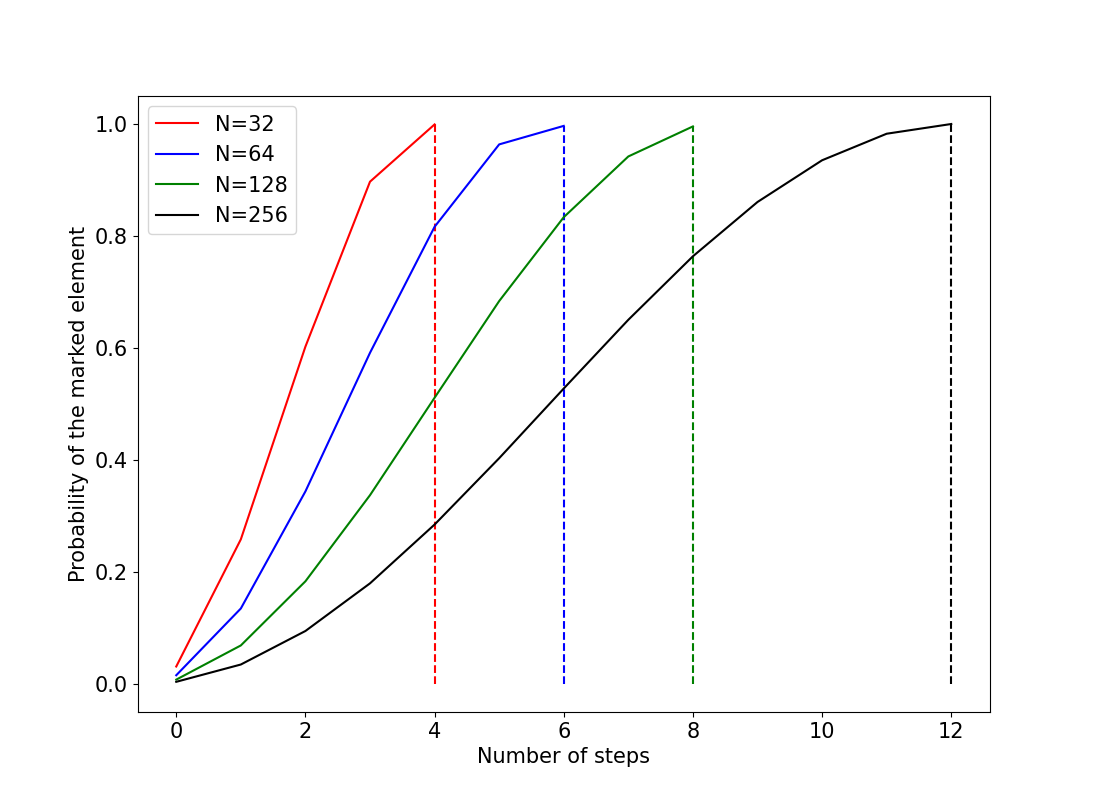
\includegraphics[scale=0.40]{img/Grover/GroverOneMarked3264128256}
	\caption{Grover one marked element temp.} 
	\label{fig:groverOneMarked163264128}
\end{figure}
The unitary evolution operator was applied approximately $\frac{\pi}{4}\sqrt{N}$ times and the amplitudes associated with those states were stored as a probability distribution. Filtering the probability of the marked element and plotting it against the number of steps, shows that the maximum is indeed reached after the said number of iterations. It also shows that the maximum probability for $N=16$ is lower than for $N=128$, which makes sense since the the probability of success is maximized for larger values of $N$.
%TODO:Talvez fazer aqui uma subseccao para separar 1 marcado de multiplos e single shot?

\subsection{Multiple marked elements}
When there's more than one element marked by the oracle, the number of iterations to achieve maximum probability changes. In fact, the latter part of this section will be used to discuss the case where one single iteration of this algorithm is enough to achieve maximum probability.\par
Firstly, one must define a set $A$ that is composed of all the marked elements and set $B$ of the remaining. The state from equation \ref{eq:groverQuantumRegister} will become
\begin{equation}
	\ket{\Psi(k,l)} =\sum_{i\in A} k\ket{i} + \sum_{x \in B}l\ket{x}.
\end{equation}
%TODO: Perceber o valor the theta again.
Assuming $t$ marked elements, iterating over this state will result in
\begin{equation}
	\ket{\Psi(\frac{N-2t}{N}k + \frac{2(N-1)}{N}l, \frac{N-2}{N}l - \frac{2}{N}k)}.
\end{equation}
Choosing an angle $\theta$ such that $sin^2\theta=\frac{t}{N}$, allows the definition of the amplitudes associated with the states after $j$ iterations 
\begin{equation}
	\begin{cases}
		k_{j} =\frac{1}{\sqrt{t}} \sin{((2j+1)\theta)} 
		\\l_{j} = \frac{1}{\sqrt{N-t}}\cos{((2j+1)\theta)}.
	\end{cases}\label{eq:groverKandJ2}
\end{equation}
%TODO: Talvez reescrever esta proxima parte. Vou resumir muito.
\begin{figure}[h]
	%TODO: Decidir que figura por aqui, como menciono em cima para Ns grandes talvez aumentar o N ou por 4 ou mais exemplos de Ns diferentes.
	%TODO: Se calhar fazer figura A e B para 2 e 3 marcados.
	\centering
	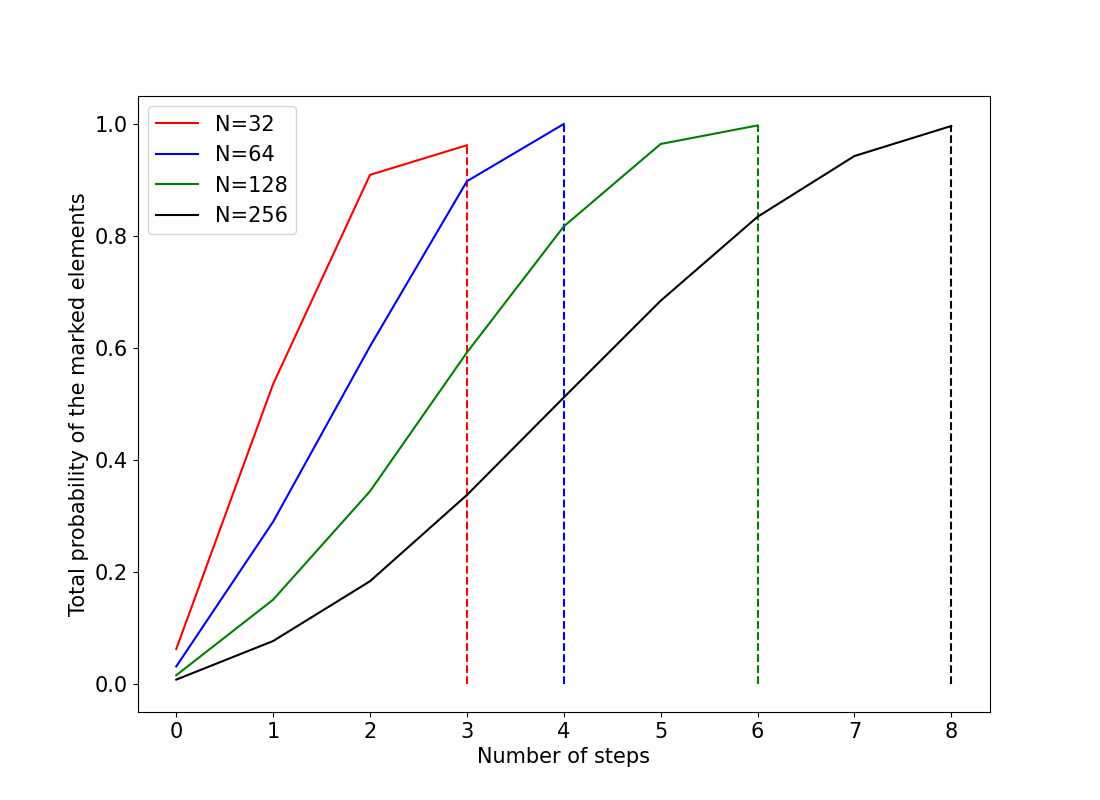
\includegraphics[scale=0.40]{img/Grover/GroverMultipleMarked3264128256}
	\caption{Grover Multiple marked temp.} 
	\label{fig:groverMultipleMarked3264128256}
\end{figure}
Similarly to the one solution case, it can be shown that setting the number of iterations $m$, to the nearest lower integer of $\frac{\pi}{4\theta}$ will result in a probability of failure $(N-t)l^2_m \leq \frac{t}{N}$. Because $\theta \geq \sin\theta = \sqrt{\frac{t}{N}}$ then
%TODO: Perceber esta transicao da prob falha para o range do valor de m.
\begin{equation}
	m \leq \frac{\pi}{4\theta} \leq \frac{\pi}{4}\sqrt{\frac{N}{t}}.
	\label{eq:multipleMarkedIterations}
\end{equation}\par
%TODO: Perceber melhor o 4thetaj no inicio da pagina 3. Sera que vale a pena mencionar?
From a more practical perspective, if one were to mark two elements of a $64$ element set, maximum probability is expected to be reached in approximately 4 steps, since $\floor{\frac{\pi}{4}\sqrt{\frac{64}{2}}} = 4$. Likewise, for $N=256$, the number of iterations is rounded to $8$, which is plotted along several other values of $N$ in figure \ref{fig:groverMultipleMarked3264128256}. The y-axis is now the sum total probability of the marked elements and the x-axis represents the range of steps that spans from $0$ to $\floor{\frac{\pi}{4}\sqrt{\frac{N}{2}}}$ for each $N$.
%:TODO: Expandir a explicacao da figura, pensar no que escrever
Again, the probability of success approaches $1$ as $N$ increases. However, comparing to figure \ref{fig:groverOneMarked163264128}, the number of iterations that maximize probability is lower for each $N$, in agreement with equation \ref{eq:multipleMarkedIterations}.
\subsection{Single-Shot Grover}
An interesting case arises when the number of marked elements is set to $t=\frac{N}{4}$, because 
\begin{equation}
	sin^2\theta = \frac{\frac{N}{4}}{N} = \frac{1}{4} \iff \sin\theta = \frac{1}{2} \iff \theta = \frac{\pi}{6}. 
	\label{eq:singleShotTheta}
\end{equation}
\begin{figure}[h]
	%TODO: Decidir que figura por aqui, como menciono em cima para Ns grandes talvez aumentar o N ou por 4 ou mais exemplos de Ns diferentes.
	%TODO: Se calhar fazer figura A e B para 2 e 3 marcados.
	\centering
	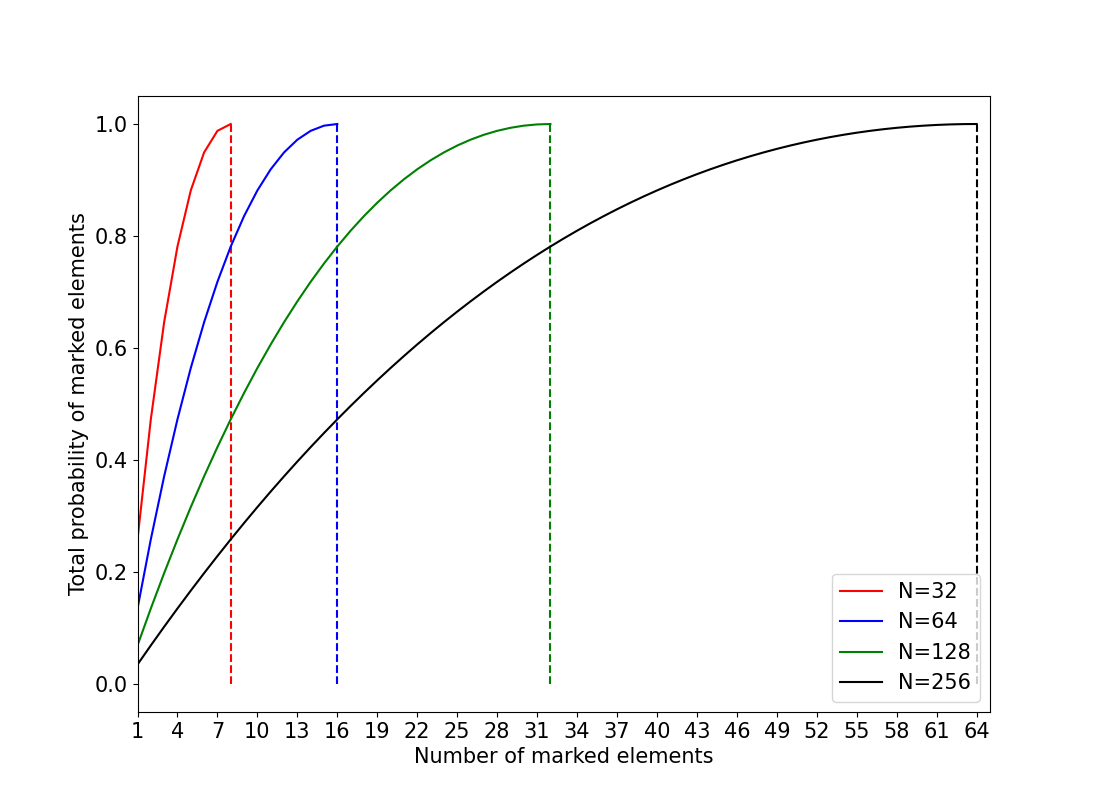
\includegraphics[scale=0.40]{img/Grover/GroverSingleShot3264128256}
	\caption{Single Shot temp} 
	\label{GroverSingleShot3264128256}
\end{figure}
Note that there are an infinite number of negative and positive solutions, but equation \ref{eq:singleShotTheta} reflects the only relevant one in this context. As a consequence, amplitudes associated with state $\ket{\Psi(k_1,l_1)}$ become 
\begin{equation}
	\begin{cases}
		k_{1} = \frac{1}{\sqrt{t}} \sin{((2+1)\theta)} = \frac{1}{\sqrt{\frac{N}{4}}} \sin{(3\frac{\pi}{6})} = \frac{2}{\sqrt{N}}
		\\l_{1} = \frac{1}{\sqrt{N-t}}\cos{((2+1)\theta)} = \frac{1}{\sqrt{N-\frac{N}{4}}}\cos{(3\frac{\pi}{6})} = 0.
	\end{cases}\label{eq:groverSingleShotKandJ}
\end{equation}
%:TODO: Escrever mais sobre a figura!
These results show that the amplitudes associated with the marked states double in relation to $\ket{\Psi_0}$ and the remaining states disappear after only one iteration. This behaviour can be seen in figure \ref{GroverSingleShot3264128256}, where the total probability of marked elements reaches $1$ once the number of marked elements is $\frac{1}{4}$ of the total elements.  
\end{document}
